\section{Method}
\label{sec:methodology}

\subsection{Overview}
\label{sec:method_overview}

We propose \textbf{YogaLLaVA V3}, a geometry-conditioned vision--language model for fine-grained yoga-pose understanding.
Given an RGB image $I$, a natural-language question $q$, and an ordered set of body measurements $\mathcal{G}$, the model generates an answer $y$ containing qualitative explanations and, when required, continuous angular values.
We formulate this task as conditional generation:
\begin{equation}
    p_{\Theta}(y\mid I,q,\mathcal{G}),
    \label{eq:problem_formulation}
\end{equation}
where $\Theta$ denotes the trainable model parameters.

As illustrated in Fig.~\ref{fig:yogallava_architecture}, YogaLLaVA V3 extends LLaVA-1.5-7B with two components for continuous geometric reasoning.
First, a geometry encoder converts ordered scalar body measurements into tokens in the language-model embedding space.
Second, an angle-regression head predicts a continuous value whenever the decoder produces an \texttt{<ANGLE>} token.
The predicted scalar is subsequently embedded back into the sequence, so that later words and angle slots condition on previously generated measurements.
The design preserves standard autoregressive language generation and does not represent angles solely as sequences of discrete text tokens.

The measurements are obtained from the SAM 3D Body reconstruction and metric extraction described in Sec.~\ref{sec:dataset}.
Accordingly, YogaLLaVA V3 reasons jointly over visual evidence, language, and supplied geometry.
It does not independently reconstruct the complete geometry vector from RGB pixels.

\begin{figure*}[!t]
    \centering
    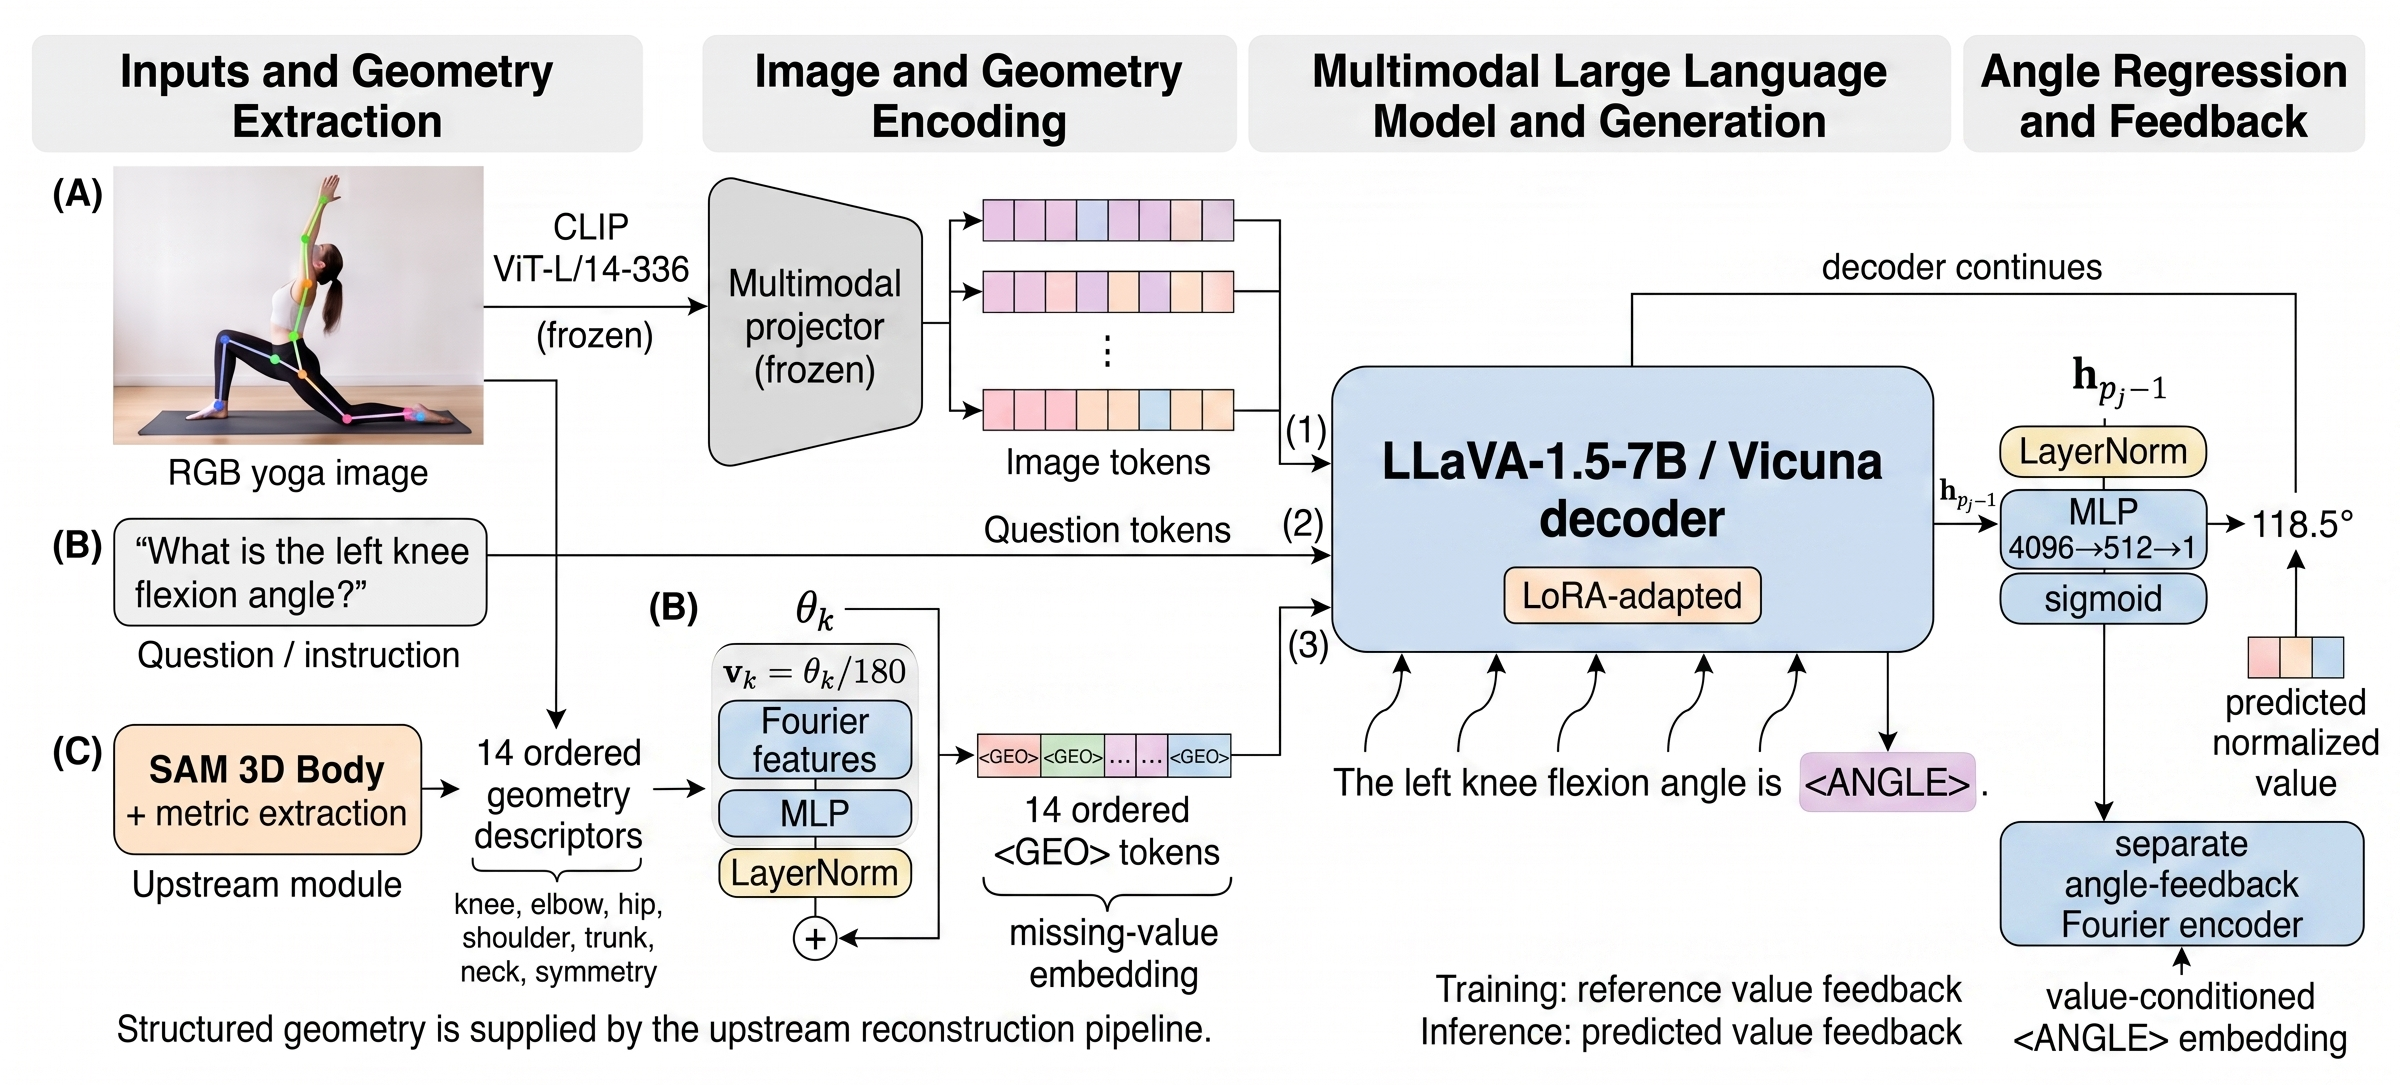
\includegraphics[width=0.98\textwidth]{method.png}
    \caption{Overview of YogaLLaVA V3. An input image is encoded by the frozen
    LLaVA vision encoder and projector, while an ordered set of degree-valued body descriptors
    is mapped to metric-aware \texttt{<GEO>} tokens. The causal language decoder
    attends jointly to visual, geometric, and textual context. When the decoder
    produces an \texttt{<ANGLE>} token, a regression head predicts the associated
    continuous value, which is embedded back into the sequence to condition
    subsequent generation.}
    \label{fig:yogallava_architecture}
\end{figure*}

\subsection{Structured Geometry Input}
\label{sec:structured_geometry_input}

YogaLLaVA V3 uses a fixed vocabulary of $K=14$ degree-valued descriptors.
The vocabulary covers left and right knee flexion, left and right elbow flexion, left and right hip opening, left and right shoulder elevation, trunk tilt, lateral trunk bend, trunk twist, neck alignment, knee symmetry, and elbow symmetry.
These descriptors form the angular subset of the broader geometric taxonomy introduced in Sec.~\ref{sec:dataset}.
Scale-dependent quantities, such as stance width and body-center offset, are not supplied to the model.
Hip symmetry is likewise not represented by a dedicated input descriptor, although three hip-symmetry targets occur in the held-out test set.

We represent the ordered geometry input as
\begin{equation}
    \mathcal{G}
    =
    \left\{(\theta_k,m_k)\right\}_{k=1}^{K},
    \qquad m_k\in\{0,1\},
    \label{eq:geometry_input}
\end{equation}
where $\theta_k$ is the $k$-th descriptor in degrees and $m_k$ indicates whether that measurement is available.
Explicitly modeling validity is necessary because a missing measurement is semantically distinct from a valid angle close to zero.

\subsection{Multimodal Geometry Representation}
\label{sec:geometry_representation}

\noindent\textbf{Visual and language inputs.}
The image is processed by the pretrained CLIP ViT-L/14-336 vision encoder in LLaVA.
Its patch-level features are projected into the language-model hidden space through the frozen multimodal projector.
The instruction and question are tokenized using the LLaVA tokenizer and combined with the projected visual features in the standard LLaVA input sequence.

To supply the geometry, we append exactly $K$ special \texttt{<GEO>} placeholders in a fixed canonical order.
Before decoding, the ordinary embeddings of these placeholders are replaced by geometry representations with the same dimensionality as the language-model hidden states.
Consequently, visual features, text tokens, and measurements are processed within a shared autoregressive sequence.

\noindent\textbf{Fourier encoding of continuous measurements.}
For every available descriptor, we normalize its value to $[0,1]$:
\begin{equation}
    v_k=\frac{\theta_k}{180}.
    \label{eq:angle_normalization}
\end{equation}
We encode $v_k$ with $B=16$ fixed, logarithmically spaced Fourier frequency bands instead of a single linear projection:
\begin{equation}
\begin{split}
    \boldsymbol{\phi}(v_k)=\big[
        &\sin(\omega_1v_k),\ldots,\sin(\omega_Bv_k),\\
        &\cos(\omega_1v_k),\ldots,\cos(\omega_Bv_k),v_k
    \big].
\end{split}
\label{eq:fourier_features}
\end{equation}
This mapping produces a $(2B+1)=33$ dimensional representation.
A two-layer MLP with hidden width 256 projects it to the $d=4096$ dimensional language-model space:
\begin{equation}
    \mathbf{z}_k
    =f_{\mathrm{geo}}\!\left(\boldsymbol{\phi}(v_k)\right),
    \qquad \mathbf{z}_k\in\mathbb{R}^{d}.
    \label{eq:scalar_projection}
\end{equation}

\noindent\textbf{Metric identity and missing values.}
The same scalar may carry different meanings for different anatomical measurements.
We therefore associate each descriptor with a learned metric-identity embedding $\mathbf{e}^{\mathrm{id}}_k\in\mathbb{R}^{d}$.
The final token for descriptor $k$ is
\begin{equation}
    \mathbf{g}_k=
    \begin{cases}
    \operatorname{LN}\!\left(
        \mathbf{e}^{\mathrm{id}}_k+\mathbf{z}_k
    \right), & m_k=1,\\[5pt]
    \operatorname{LN}\!\left(
        \mathbf{e}^{\mathrm{id}}_k+\mathbf{e}^{\mathrm{miss}}
    \right), & m_k=0,
    \end{cases}
    \label{eq:geometry_token}
\end{equation}
where $\mathbf{e}^{\mathrm{miss}}\in\mathbb{R}^{d}$ is a learned missing-value embedding and $\operatorname{LN}$ denotes layer normalization.
The ordered geometry sequence is
\begin{equation}
    \mathbf{G}=[\mathbf{g}_1,\ldots,\mathbf{g}_K]
    \in\mathbb{R}^{K\times d}.
    \label{eq:geometry_sequence}
\end{equation}
These vectors replace the corresponding \texttt{<GEO>} embeddings.
The decoder attends jointly to the image, question, and metric-specific continuous geometry.

\subsection{Angle-Aware Language Generation}
\label{sec:angle_generation}

Standard language models express numbers through discrete subword tokens.
Subword generation provides no explicit continuous prediction objective.
YogaLLaVA V3 instead introduces a special \texttt{<ANGLE>} token that separates numeric-slot placement from scalar-value estimation.
During training, every degree value in a geometry-grounded answer is replaced by \texttt{<ANGLE>}, and its normalized value is retained as a continuous target aligned with that token position.
For example,
\begin{quote}
\small
\textit{The left knee flexion angle is $140.2^\circ$.}
\end{quote}
is represented internally as
\begin{quote}
\small
\texttt{The left knee flexion angle is <ANGLE>.}
\end{quote}
The language decoder thus learns \emph{where} an angular value is required, whereas the regression branch learns \emph{which} value should occupy that position.

Let $p_j$ denote the position of the $j$-th \texttt{<ANGLE>} token.
Under causal decoding, the hidden state $\mathbf{h}_{p_j-1}$ produces the token at position $p_j$.
We predict its normalized value as
\begin{equation}
    \widehat{v}_j
    =\sigma\!\left(
        f_{\mathrm{reg}}(\mathbf{h}_{p_j-1})
    \right),
    \label{eq:angle_regression}
\end{equation}
where $f_{\mathrm{reg}}$ comprises layer normalization, a $4096\!\rightarrow\!512$ linear layer, GELU, and a $512\!\rightarrow\!1$ linear layer.
The sigmoid restricts predictions to $[0,1]$, after which the angle is recovered in degrees:
\begin{equation}
    \widehat{\theta}_j=180\widehat{v}_j.
    \label{eq:angle_denormalization}
\end{equation}
Using $\mathbf{h}_{p_j-1}$ ensures that the current value is estimated from the preceding causal context.
No value-conditioned embedding is placed at the current \texttt{<ANGLE>} position.

\noindent\textbf{Continuous-value feedback.}
After an angle slot is produced, its scalar value is re-embedded into the sequence so that subsequent language and later angle slots may condition on it.
An independent scalar encoder defines
\begin{equation}
    \mathbf{a}(u_j)
    =\mathbf{e}^{\mathrm{angle}}
    +f_{\mathrm{slot}}\!\left(\boldsymbol{\phi}(u_j)\right),
    \label{eq:angle_feedback}
\end{equation}
where $\mathbf{e}^{\mathrm{angle}}$ is a learned base embedding and $f_{\mathrm{slot}}$ is distinct from the geometry-input encoder $f_{\mathrm{geo}}$.
During teacher-forced training, $u_j$ is the reference normalized angle.
During autoregressive inference, $u_j=\widehat{v}_j$.
Accordingly, subsequent tokens condition on the reference value during training and on the model's own prediction at inference time.

\subsection{Joint Language and Geometry Learning}
\label{sec:training_objective}

We jointly optimize natural-language generation and continuous angle prediction.
Language supervision is restricted to the assistant response.
Image and geometry placeholders, the instruction, the question, and padding positions are excluded.
Let $\mathcal{T}$ denote the supervised assistant-token positions.
The causal language-modeling objective is
\begin{equation}
    \mathcal{L}_{\mathrm{LM}}
    =-\frac{1}{|\mathcal{T}|}
    \sum_{t\in\mathcal{T}}
    \log p_{\Theta}\!\left(
        y_t\mid y_{<t},I,q,\mathcal{G}
    \right).
    \label{eq:language_loss}
\end{equation}

For a minibatch containing $N$ supervised angle slots, the regression branch is optimized in normalized angle space using
\begin{equation}
    \mathcal{L}_{\mathrm{ang}}
    =\frac{1}{N}\sum_{j=1}^{N}
    \operatorname{SmoothL1}_{\beta}
    \!\left(\widehat{v}_j-v_j\right).
    \label{eq:regression_loss}
\end{equation}
The complete training objective is
\begin{equation}
    \mathcal{L}
    =\mathcal{L}_{\mathrm{LM}}
    +\lambda_{\mathrm{ang}}\mathcal{L}_{\mathrm{ang}},
    \label{eq:total_loss}
\end{equation}
with $\lambda_{\mathrm{ang}}=0.75$ and $\beta=0.05$, corresponding to a $9^\circ$ SmoothL1 transition in degree space.
The language term is causal cross-entropy with label smoothing.
Domain-knowledge records contain no \texttt{<ANGLE>} positions and therefore contribute only $\mathcal{L}_{\mathrm{LM}}$.

As a regularizer, we apply full geometry dropout to 15\% of geometry-grounded training records.
For a selected record, every measurement is marked unavailable and represented by the learned missing-value embedding.
We do not evaluate behavior under missing measurements at test time.

The CLIP vision encoder and multimodal projector remain frozen.
We adapt the Vicuna language decoder using LoRA with rank 32, scaling parameter 64, and dropout 0.10.
LoRA is applied to the $q$, $k$, $v$, and $o$ attention projections and to the gate, up, and down feed-forward projections.
The geometry encoder, angle-feedback encoder, learned angle embedding, regression head, and LoRA parameters are optimized jointly.
After adding \texttt{<GEO>} and \texttt{<ANGLE>} to the vocabulary, the input-embedding matrix and language-model output projection are also trainable.

\subsection{Autoregressive Inference}
\label{sec:inference}

At inference time, SAM 3D Body reconstruction provides the ordered geometry descriptors, while the frozen LLaVA vision encoder and projector process the input image.
The image, geometry tokens, instruction, and question are supplied without a reference answer.

Decoding proceeds autoregressively.
Ordinary tokens follow the standard LLaVA generation process.
When \texttt{<ANGLE>} is selected, the hidden state that produced it is passed to the regression head to obtain $\widehat{v}_j$.
The prediction is converted to degrees for the final response and encoded through Eq.~\eqref{eq:angle_feedback} as the embedding of that \texttt{<ANGLE>} token before decoding resumes.
After generation, the placeholders are replaced in order by their predicted degree values.
Token probabilities and scalar predictions are not averaged or combined at the output level.
The two interact through the slot-placement and continuous-value feedback mechanism.
